%% Preamble
  \documentclass{homework}

  \hwTitle{Assignment\ \#2 - Integral Calculus} % Assignment title
  \hwDueDate{Friday,\ May\ 17,\ 2013} % Due date
  \hwClass{Physics\ 441} % Course/class
  % \hwInstructor{Manuel Berrondo} % Teacher/lecturer
  \hwAuthor{Spencer Lyon} % Your name

% New commands I use a lot
  \newcommand{\bs}[1]{\ensuremath{\boldsymbol{#1}}}
  \newcommand{\bhat}[1]{\ensuremath{\boldsymbol{\hat{#1}}}}
  \newcommand{\cross}[2]{\ensuremath{\boldsymbol{#1} \times \boldsymbol{#2}}}
  \newcommand{\curl}[1]{\ensuremath{\cross{\nabla}{\bs{#1}}}}
  \newcommand{\diver}[1]{\ensuremath{\nabla \times \bs{#1}}}

  % partial derivative as a fraction
  \newcommand{\fracpd}[2]{
    \ensuremath{\frac{\partial #1}{\partial #2}}
  }

  % Just a vector in xhat yhat zhat
   \newcommand{\xyzvec}[3]{
   \ensuremath{
      (#1) \bhat{x} + (#2) \bhat{y} + (#3) \bhat{z}
   }
   }

   % Represents vec \cdot dl
   \newcommand{\dotdl}[3]{
   \ensuremath{
      (#1) \partial x+ (#2) \partial y + (#3) \partial z
   }
   }

   % Just a vector in shat phihat zhat
   \newcommand{\sphizvec}[3]{
   \ensuremath{
      (#1) \bhat{s} + #2 \bhat{\phi} + (#3) \bhat{z}
   }
   }

   % Express integral bounds with right arrow
   \newcommand{\arrowbounds}[3]{
   \ensuremath{
      #1: #2 \rightarrow #3
   }
   }

  % Express integral bounds in parenthesis with tall vertical bar
   \newcommand{\intbounds}[3]{
   \ensuremath{
      \left. \left( #1 \right) \right|_{#2}^{#3}
   }
   }




\begin{document}

\maketitle

\begin{homeworkProblem}[Problem 1.25]
  Using vectors $$ \bs{A} = \xyzvec{x}{2y}{3z} \qquad \bs{B} = \xyzvec{3y}{-2x}{0}$$ Check the following identities:

  \begin{enumerate}
    \item $\nabla \cdot (\cross{\bs{A}}{\bs{B}}) = \bs{B} \cdot (\cross{\nabla}{\bs{A}}) + \bs{A} \cdot (\cross{\nabla}{\bs{B}})$
    \item $\nabla(\bs{A} \cdot \bs{B}) = \cross{\bs{A}}{(\cross{\nabla}{\bs{B}})} + \cross{\bs{B}}{(\cross{\nabla}{\bs{A}}}) + (\bs{A} \cdot \nabla) \bs{B} + (\bs{B} \cdot \nabla) \bs{A}$
    \item $\cross{\nabla}{(\cross{\bs{A}}{\bs{B}})} = (\bs{B} \cdot \nabla)\bs{A} -(\bs{A} \cdot \nabla)\bs{B} + \bs{A}(\nabla \cdot \bs{B}) - \bs{B}(\nabla \cdot \bs{A})$
  \end{enumerate}
  \vspace{.2in}

  \problemAnswer{ % Answer
    For this problem we will use the following definitions:

    \begin{itemize}
      \item \curl{A} = $\xyzvec{0}{0}{0}$
      \item \curl{B} = $\xyzvec{0}{0}{-5}$
      \item \diver{A} = $6$
      \item \diver{B} = $0$
      \item $\cross{A}{B} = \xyzvec{6 x z}{9 y z}{- 2 x^{2} - 6 y^{2}}$
      \item  $\bs{A} \cdot \bs{B} = - xy$
    \end{itemize}

    We will now verify each of the identities:

    \begin{enumerate}
      \item
        \begin{align*}
          15 z = \nabla \cdot (\cross{\bs{A}}{\bs{B}}) &= \bs{B} \cdot (\cross{\nabla}{\bs{A}}) - \bs{A} \cdot (\cross{\nabla}{\bs{B}}) \\
            &= \bs{B} \cdot \left(\xyzvec{0}{0}{0} \right) - \bs{A} \cdot \left( \xyzvec{0}{0}{-5} \right)\\
            &= 0 - (-15 z)\\
            &= 15z \qed
        \end{align*}
      \item Below I make the following substitutions:
      \begin{itemize}
        \item $\bs{A} \times [\xyzvec{0}{0}{-5}] = \xyzvec{-10y}{5x}{0}$
        \item $\bs{B} \times [\xyzvec{0}{0}{0}] = 0$
        \item  $(\bs{A} \cdot \nabla) \bs{B} = \xyzvec{6y}{-2x}{0}$
        \item $ (\bs{B} \cdot \nabla) \bs{A} = \xyzvec{3y}{-4x}{0}$
      \end{itemize}

      \begin{align*}
        \xyzvec{- y}{- x}{0} = \nabla(\bs{A} \cdot \bs{B}) &= \cross{\bs{A}}{(\cross{\nabla}{\bs{B}})} + \cross{\bs{B}}{(\cross{\nabla}{\bs{A}}}) + (\bs{A} \cdot \nabla) \bs{B} + (\bs{B} \cdot \nabla) \bs{A}\\
          &= \xyzvec{-10y}{5x}{0}+ 0 + \xyzvec{6y}{-2x}{0} + \xyzvec{3y}{-4x}{0}\\
          &= \xyzvec{-y}{-x}{0} \qed
      \end{align*}
      \item Below I make the following substitution (as well as some from the previous part): $\nabla \times (\cross{A}{B}) = \xyzvec{- 21 y}{10 x}{0}$.

      \begin{align*}
         \xyzvec{- 21 y}{10 x}{0} =\nabla \times (\cross{A}{B}) &= (\bs{B} \cdot \nabla)\bs{A} -(\bs{A} \cdot \nabla)\bs{B} + \bs{A}(\nabla \cdot \bs{B}) - \bs{B}(\nabla \cdot \bs{A}) \\
          &= \xyzvec{3y}{-4x}{0} - \xyzvec{6y}{-2x}{0} + \bs{A} (0) + \bs{B} (6) \\
          &= \xyzvec{3y}{-4x}{0} - \xyzvec{6y}{-2x}{0} + \xyzvec{18 y}{- 12 x}{0}\\
          &= \xyzvec{- 21 y}{10 x}{0} \qed
      \end{align*}
    \end{enumerate}


  }
\end{homeworkProblem}

\begin{homeworkProblem}[Problem 1.27]
  Prove that the divergence of a curl is always zero. Check it for $$\bs{v} = \xyzvec{x^2}{3xz^2}{-2xz}$$
  \vspace{.2in}
  \problemAnswer{ % Answer

    The general form for the curl of a vector function is $$\nabla \times \bs{F}(x, y, z) =  \left( \fracpd{F_z}{y} - \fracpd{F_y}{z}\right) \bhat{x} - \left(\fracpd{F_x}{z} - \fracpd{F_z}{x} \right) \bhat{y} +  \left(\fracpd{F_x}{y} - \fracpd{F_y}{x} \right) \bhat{z}$$

    Taking the divergence of this we get:
      \begin{align*}
        \nabla \cdot \left(\nabla \times \bs{F}(x, y, z) \right) &= \nabla \cdot \left[ \left( \fracpd{F_z}{y} - \fracpd{F_y}{z}\right) \bhat{x} - \left(\fracpd{F_x}{z} - \fracpd{F_z}{x} \right) \bhat{y} +  \left(\fracpd{F_x}{y} - \fracpd{F_y}{x} \right) \bhat{z} \right] \\
          &= \fracpd{ }{x}  \left( \fracpd{F_z}{y} - \fracpd{F_y}{z}\right)  - \fracpd{ }{y} \left(\fracpd{F_x}{z} - \fracpd{F_z}{x} \right) + \fracpd{ }{z} \left(\fracpd{F_x}{y} - \fracpd{F_y}{x} \right) \\
          &= \left[ \fracpd{ ^2F_z}{x \partial y} - \fracpd{ ^2F_z}{y \partial x} \right] + \left[ \fracpd{ ^2F_y}{x \partial z} - \fracpd{ ^2F_y}{z \partial x} \right] + \left[ \fracpd{ ^2F_x}{z \partial y} - \fracpd{ ^2F_x}{y \partial z} \right]
          &= 0 + 0 + 0 = 0 \qed
      \end{align*}

      Now I will verify using the vector $\bs{v}$

      \begin{align*}
        \nabla \cdot (\cross{\nabla}{v}) & = \nabla \cdot \left(\xyzvec{- 6 x z}{2 z}{3 z^{2}} \right) \\
          &=  \fracpd{ }{x} \left[ - 6 x z \right] + \fracpd{ }{y} \left[ 2 z \right] + \fracpd{ }{z} \left[ 3 z^{2} \right] \\
          &= -6z + (6z) = 0 \qed
      \end{align*}

  }
\end{homeworkProblem}

\begin{homeworkProblem}[Problem 1.32]
  Check the fundamental theorem for gradients, using $T = x^2 + 4xy + 2yz^3$, the points $\bs{a} = (0,0,0), \bs{b}=(1,1,1)$, and the three paths in Figure \ref{fig:threepaths}. The paths are:

  \begin{enumerate}
    \item $(0, 0, 0) \rightarrow (1, 0 ,0) \rightarrow (1, 1, 0) \rightarrow (1, 1, 1)$
    \item $(0, 0, 0) \rightarrow (0, 0 ,1) \rightarrow (0, 1, 1) \rightarrow (1, 1, 1)$
    \item The parabolic path $z = x^2, y = x$
  \end{enumerate}

  \begin{figure}[!h]
      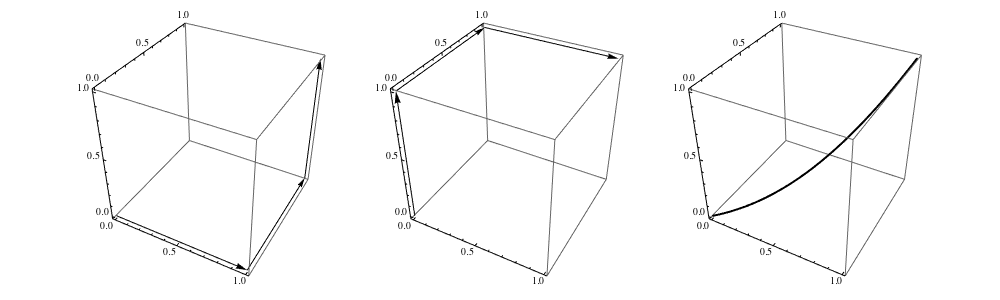
\includegraphics[width=\linewidth, height=2in]{paths.png}
      \caption{The three paths for problem 1.32}
      \label{fig:threepaths}
  \end{figure}

  \vspace{.2in}

  \problemAnswer{ % Answer

  We first start with $$\nabla T = \xyzvec{2x + 4y}{4x + 2z^3}{6yz^2}$$ We will be integrating $$\nabla T \cdot dl = \dotdl{2x + 4y}{4x + 2z^3}{6yz^2}$$

  \begin{enumerate}
    \item The three integrals below represent the three segments.
      \begin{itemize}
        \item $y=z=\partial y=\partial z= 0$  $x$ from $0$ to $1$:  $\int_0^1 (2x + 4[y=0]) dx = x^2|_0^1 = 1$
        \item $x=1$, $\partial x= \partial z = z = 0$, and we integrate $y$ from $0$ to $1$: $\int_0^1  (4[x=1] + 2[z=0]^3) dy = 4y|_0^1 = 4$
        \item $x=y=1$, $dx=dy=0$ and we integrate $z$ from $0$ to  $1$: $\int_0^1 (6[y=1] z^2) dz = 2z^3|_0^1 = 2$
      \end{itemize}
      Putting them together we get that $\int_a^b \nabla T \cdot dl = 1 + 4 + 2 = 7$
    \item
       \begin{itemize}
        \item $y=x=dy=dx= 0$  $z$ from $0$ to $1$:  $\int_0^1 (6[y=0] z^2) dz =  0$
        \item $z=1$, $dx= dz = x = 0$, and we integrate $y$ from $0$ to $1$: $\int_0^1  (4[x=0] + 2[z=1]^3) dy = 2y|_0^1 = 2$
        \item $z=y=1$, $dz=dy=0$ and we integrate $x$ from $0$ to  $1$: $\int_0^1  (2x + 4[y=1]) dx = x^2|_0^
        1 + 4 = 5$
      \end{itemize}
      Putting them together we get that $\int_a^b \nabla T \cdot dl = 0 + 2 + 5 = 7$
    \item We do this one in a single shot be replacing all $y$ and $z$ terms in $\nabla T \cdot dl$ with terms of only $x$. We need to remember that $y = x$ and $z = x^2$. That makes $dy = dx$ and $dz = 2 dx$.
      \begin{align*}
        \nabla T \cdot dl &= (2x + 4x)dx + (4x + 2x^6) dx + (3x^4)2dx \\
          &= (10x + 14x^6) dx
      \end{align*}
    Now I can integrate $x$ from $0$ to  $1$:
    \begin{align*}
      \int_0^1 (10x + 14x^6) dx &= \left. \left[5x^2 + 2^7 \right] \right|_0^1 \\
        &= 2 + 5 = 7
    \end{align*}
    These are all the same so we have verified the fundamental theorem for gradients for this function along the given paths. \qed
  \end{enumerate}

  }
\end{homeworkProblem}

\begin{homeworkProblem}[Problem 1.34]
  Test Stokes' theorem for the function $\bs{v} = \xyzvec{xy}{2yz}{3zx}$ using the triangular region defined by the points $(0, 0, 0), (0, 0, 2), \text{ and } (0, 2, 0)$ that moves in the counter clockwise direction..
  \vspace{.2in}

  \problemAnswer{ % Answer

  Stokes' theorem gives the following: $$ \int_S (\curl{v}) \cdot d\bs{a} = \oint_{\mathbb{P}} \bs{v} \cdot d \bs{l}$$

  We will need to know that $\curl{v} = \xyzvec{-2y}{-3z}{-x}$.

  Also, from the rotation of the curve, we can say that $d\bs{a}$ is oriented in the $\bhat{x}$ direction. With that we can say that $d\bs{a} = (dy dz) \bhat{x}$.

  We can finally say that $(\curl{v}) \cdot d\bs{a} = -2y dy dz$

  We need to evaluate the integral $\int_S (\curl{v}) \cdot d\bs{a}$, but before we can to that we need to define the bounds of integration for the integrals in $y$ and $z$. A simple way to do this is to write $y$ as a function of z using the expression $$y = 2 - z$$. The bounds of integration then become $0$ to $ z- 2$ for $y$ and $0$ to $2$ for z.

  \begin{align*}
     \int_S (\curl{v}) \cdot d\bs{a} &= \int_0^2\left(\int_0^{z-2} -2y dy\right) dz \\
       &= \int_0^2 \left( -y^2|_0^{z-2} \right) dz \\
       &= \int_0^2 - (2 - z)^2 dz \\
       &= - \int_0^2 (z^2 - 4z + 4) dz \\
       &= - \left[ \frac{1}{3} z^3 - 2z^2 + 4z \right] |_0^2 \\
       &= - \left(\frac{8}{3} -8 + 8 \right) = \frac{8}{3}
  \end{align*}

  To verify this we need to check that $\oint_{\mathbb{P}} \bs{v} \cdot d \bs{l} = \frac{8}{3}$. To do this we need to know that $\bs{v} \cdot d \bs{l} = (xy) dx + (2yz) dy + (3zx) dz$ I will break the integral into three sections, each representing one leg of the triangle.

  \begin{enumerate}
    \item Bottom leg: $x=z=dx=dz=0$ and $y$ goes from $0$ to $2$. Plugging zeros in we see that $\bs{v} \cdot d \bs{l} = 0$, therefore the integral for this section in $0$.
    \item Hypotenuse: $x=dx=0$, $z = 2-y$, $dz = -dy$, and $y$ goes from $2$ to $0$. Plugging things in we see that $\bs{v} \cdot d \bs{l} = (2yz)dy = (2y(2-y))dy$
    \begin{align*}
      \int_2^0 (2y(2-y))dy &= \int_2^0 4y - y^2 dy \\
        &=  - \int_0^2 4y - y^2 dy \\
        &= - \left. \left(2y^2 - \frac{2}{3} y^3 \right) \right|_0^2 \\
        &= -(8 - \frac{16}{3}) = -\frac{8}{3}
    \end{align*}
    \item Vertical leg: $x=dx=y=dy=0$.  $z$ goes from $2$ to $0$. Plugging zeros in we see that $\bs{v} \cdot d \bs{l} = 0$, therefore the integral for this section in $0$.
  \end{enumerate}

  Putting all three pieces together we see that the line integral way gave us $0 -\frac{8}{3} + 0 = -\frac{8}{3}$, which is what we got above. \qed
  }
\end{homeworkProblem}

\begin{homeworkProblem}[Problem 1.43]

  \begin{enumerate}
    \item  find the divergence of the function $$\bs{v} = \sphizvec{s(2 + \sin^2(\phi))} {s \sin\phi \cos\phi} {3z}$$
    \item Test the divergence theorem for this function, using the quarter of radius 2, height 5 defined in the first quadrant of the x-y plane.
    \item Find the curl of \bs{v}.
  \end{enumerate}

  \vspace{.2in}

  \problemAnswer{ % Answer
    \begin{enumerate}
      \item From the book we can get that the divergence in spherical coordinates is equal to: $$\frac{1}{s} \fracpd{}{s} (s v_s) + \frac{1}{s} \fracpd{v_{\phi}}{\phi} + \fracpd{v_z}{z} $$ Applying that to our function we get
        \begin{align*}
          \nabla \cdot \bs{v} &= \frac{1}{s} \fracpd{}{s} (s s(2 + \sin^2(\phi))) + \frac{1}{s} \fracpd{(s \sin\phi \cos\phi)}{\phi} + \fracpd{3z}{z} \\
            &=\frac{1}{s} 2s \left(2 + \sin^2 \phi \right) + \frac{1}{s} s \left(\cos^2 \phi - \sin^2 \phi \right) + 3 \\
            &= 4 + 2 \sin^2 \phi  + \cos^2 \phi - \sin^2 \phi + 3 \\
            &= 4 + \cos^2 \phi + \sin^2 \phi + 3 \\
            &= 4 + 1 + 3 = 8
        \end{align*}
      \item We need to show that the two sides of the integral are equal. The first is easy.
        \begin{align*}
          \int\nabla \cdot \bs{v} d \tau &= \int_0^2 \int_0 ^{\pi/2} \int_0^5  8 s ds d\phi dz \\
            &= 8 \left. \left( \frac{s^2}{2} \right) \right|_0^2 \left. \left( \phi \right) \right|_0^{\pi/2} \left. \left( z \right) \right|_0^5 \\
            &= 40 \pi
        \end{align*}

        Now for the hard part... We need to integrate over all 5 pieces of the surface (top, bottom, left, right, curved).
        \begin{enumerate}
          \item Top: $z=5$, where $\arrowbounds{\phi}{0}{\pi/2}$ and $\arrowbounds{s}{0}{2}$. We also need to know that $\bs{v} \cdot d \bs{a} = 3z s ds d \phi$
            \begin{align*}
              \int \bs{v} \cdot d\bs{a} &= \int_0^2 \int_0 ^{\pi/2} 3 (z=5) s ds d \phi \\
                &= 15 \left. \left( \frac{s^2}{2} \right) \right|_0^2 \left. \left( \phi \right) \right|_0^{\pi/2} = 15 \pi
            \end{align*}
          \item Left: $\phi = \pi/2$, where $\arrowbounds{z}{0}{5}$ and $\arrowbounds{s}{0}{2}$. We also need to know that $\bs{v} \cdot d \bs{a} = s \sin \phi \cos \phi ds dz= 0$. That makes the integral for this part equal to 0.
          \item Bottom: $z=0$, where $\arrowbounds{\phi}{0}{\pi/2}$ and $\arrowbounds{s}{0}{2}$. We also need to know that $\bs{v} \cdot d \bs{a} = -3(z=0) s ds d \phi = 0$. This makes the integral for this part equal to 0.
          \item Right: Left: $\phi = 0$, where $\arrowbounds{z}{0}{5}$ and $\arrowbounds{s}{0}{2}$. We also need to know that $\bs{v} \cdot d \bs{a} =- s \sin \phi \cos \phi ds dz= 0$. That makes the integral for this part equal to 0.
          \item Curved part: $s=2$, where $\arrowbounds{\phi}{0}{\pi/2}$ and $\arrowbounds{z}{0}{5}$. We also need to know that $\bs{v} \cdot d \bs{a} = (s=2) (2 + \sin^2 \phi)(s=2) dz d \phi = 4 (2 + \sin^2 \phi) dz d \phi$
            \begin{align*}
              \int \bs{v} \cdot d\bs{a} &= \int_0^5 \int_0 ^{\pi/2} 4 (2 + \sin^2 \phi) dz d \phi \\
                &= \intbounds{\frac{5 x}{2}-\frac{1}{4} \sin (2 x)}{0}{\pi/2} \intbounds{z}{0}{5} =25 \pi
            \end{align*}
        \end{enumerate}

        Putting all these pieces together we get that the integral is $15 \pi + 0 + 0 + 0 + 25 \pi = 40 \pi$, which is the same thing we got doing the integral the other way.

      \item We now find the curl of $\bs{v}$ using the expression for the curl in spherical coordinates that we find in the book.
        \begin{align*}
          \curl{v} &= \left(\frac{1}{s} \fracpd{v_z}{\phi}  - \fracpd{v_{\phi}}{z} \right) \bhat{s} + \left(\fracpd{v_s}{z} - \fracpd{v_z}{s} \right) \bhat{\phi} + \frac{1}{s} \left[ \fracpd{}{s} (s v_{\phi} - \fracpd{v_s}{\phi} \right] \bhat{z} \\
            &= (0 - 0) \bhat{s} + (0 - 0) \bhat{y} + \frac{1}{s} \left[ 2 s \sin\phi \cos\phi  - 2 s \sin\phi \cos\phi \right] \bhat{z}= 0 \qed
        \end{align*}
    \end{enumerate}
  }
\end{homeworkProblem}

\begin{homeworkProblem}[Problem 1.45]

  Evaluate the following integrals

  \begin{enumerate}
    \item $\int_{-2}^2 (2x + 3 )\delta (3x) dx$
    \item $\int_0^2 (x^3 + 3x + 2) \delta(1 - x) dx$
    \item $\int_{-1}^1 9x^2 \delta(3x + 1) dx$
    \item $\int_{-\infty}^a \delta(x-b) dx$
  \end{enumerate}

  \vspace{.2in}

  \problemAnswer{ % Answer

  For this problem we simply use various properties of the delta distribution that we can find the in book.

    \begin{enumerate}
      \item For this part we use: $\int_{-\infty}^{\infty} f(x) \delta(kx) = \int_{\infty}^{\infty}  \left [\frac{1}{|k|} \delta(x) \right]$
        \begin{align*}
         \int_{-2}^2 (2x + 3 )\delta (3x) dx & =\int_{-2}^2 (2x + 3) \frac{1}{3}\delta (x) dx\\
           & = \frac{1}{3} [2(x=0) + 3] \\
           &= \frac{1}{3} (0 + 3) = 1
        \end{align*}
      \item For this part we use the above property and:  $f(x) \delta(x-b) = f(b)$
        \begin{align*}
         \int_0^2 (x^3 + 3x + 2) \delta(1 - x) dx &= \int_0^2 (x^3 + 3x + 2) \delta(-1[x - 1]) dx \\
           &= \int_0^2 (x^3 + 3x + 2) \delta(x- 1) dx \\
           &= [x=1]^2 + 3[x=1] + 2 = 6
        \end{align*}
      \item For this part we use the same properties as the previous part
        \begin{align*}
         \int_{-1}^1 9x^2 \delta(3x + 1) dx &= \int_{-1}^1 9x^2 \delta(3[x + 1/3]) dx \\
          &=\int_{-1}^1 9x^2  \frac{1}{3} \delta(x + 1/3) dx \\
          &=9(x=-1/3)^2 (1/3) = 1/3
        \end{align*}
      \item This one is a bit tricky, but it equal to the following:
          $$\int_{-\infty}^a \delta(x-b) dx = \begin{cases} 1 & \text{if } a > b \\ 0       & \text{otherwise}  \end{cases} \qed$$
    \end{enumerate}
  }
\end{homeworkProblem}

\begin{homeworkProblem}[Problem 1.49]

  Evaluate the integral $$J = \int_{\mathbb{V}} e^{-r} \cdot \left(\nabla \cdot \frac{\bhat{r}}{r^2}\right) d \tau$$ (where $\mathbb{V}$ is a sphere of radius $R$ , centered at the origin) by two different methods as in Ex. 1.16
  \vspace{.2in}

  \problemAnswer{ % Answer

    We will follow the same course that Example 1.16 did:

    \begin{enumerate}
      \item We begin by re-writing the divergence: $$\nabla \cdot \frac{\bhat{r}}{r^2} = 4 \pi \delta^3 (\bs{r})$$ We can now evaluate the integral
        \begin{align*}
          J &= \int_{\mathbb{V}} e^{-r} \cdot \left(\nabla \cdot \frac{\bhat{r}}{r^2}\right) d \tau \\
            &= \int_{\mathbb{V}} e^{-r}  4 \pi \delta^3 (\bs{r}) d \tau \\
            &= 4 \pi e^{-0} = 4 \pi
        \end{align*}
      \item To do this part we move the derivative term over to the $e^{-r}$ and then finish it out. Note that we use $d \bs{a} = r^2 sin \theta d \theta d \phi \bhat{r}$ and $d  \tau = 4 \pi r^2 d r $
        \begin{align*}
          J &= \int_{\mathbb{V}} e^{-r} \cdot \left(\nabla \cdot \frac{\bhat{r}}{r^2}\right) d \tau \\
            &= - \int_{\mathbb{V}} \frac{\bhat{r}}{r^2} \cdot \left[\nabla e^{-r} \right]  d \tau +\oint_{\mathbb{S}} e^{-r} \frac{\bhat{r}}{r^2} \cdot d \bs{a} \\
            &=  \int \frac{1}{r^2} e^{-r} 4 \pi r^2 dr + \int e^{-r}  \frac{\bhat{r}}{r^2} \cdot r^2 sin \theta d \theta d \phi \bhat{r} \\
            &= 4 \pi \int_0^{\infty} e^{-r}dr + e^{-R} \int sin \theta d \theta d \phi \\
            &= 4 \pi \intbounds{-e^{-r}}{0}{\infty} + 4\pi e^{-R} = 4 \pi
        \end{align*}
    \end{enumerate}

    Those two integrals gave us the same answer so we are done. \qed

  }
\end{homeworkProblem}

\begin{homeworkProblem}[Problem 1.63]

  \begin{enumerate}
    \item Find the divergence of the function $$\bs{v} = \frac{\bhat{r}}{r}.$$  First compute it directly, as in Eq 1.84. Test your result using the divergence theorem as in Eq 1.85. Is there a delta function at the origin, as there was for $\frac{\bhat{r}}{r^2}$? What is the general formula for the divergence of $r^n \bhat{r}$? [\textit{Answer}: $\nabla \cdot (r^n\bhat{r})
     = (n + 2) r^{n-1}$, unless $n = -2$, in which case it is $4\pi \delta^3(\bs{r})$; for $n<- 2$, the divergence is ill-defined at the origin.]
    \item Find the \textit{curl} of $r^n \bhat{r}$. Test your colclusion using problem 1.61b [\textit{Answer:} $\nabla \times (r^n \bhat{r}) =0$]
  \end{enumerate}

  \vspace{.2in}

  \problemAnswer{ % Answer
     \begin{enumerate}
       \item We now find the divergence using the expression for divergence in spherical coordinates.
         \begin{align*}
           \nabla \cdot \bs{v} &= \frac{1}{r^2} \fracpd{}{r} \left(r^2 \left[v_r = \frac{1}{r} \right] \right)  + 0 \bhat{\theta} + 0 \bhat{\phi}\\
            &= \frac{1}{r^2} \fracpd{r}{r}\\
            &= \frac{1}{r^2}
         \end{align*}

         Recall that the divergence theorem states that
         $$\int (\nabla \cdot \bs{A}) d \tau = \oint \bs{A} \cdot d \bs{a} $$
         We now use the divergence theorem to verify our result.  Note that we follow equation 1.85 in using $d \bs{a} = R^2 sin \theta d \theta d \phi \bhat{r}$ and $d \tau = r^2 \sin \theta dr d \theta d \phi$

         \begin{align*}
            \int (\nabla \cdot \bs{v}) d \tau &= \int \frac{1}{r^2}  r^2 \sin \theta dr d \theta d \phi \\
              &= \int_0^R \int_0^{\pi} \int_0^{2 \pi} dr \sin \theta d \theta d \phi \\
              &= 4 \pi R
         \end{align*}

          We now verify that this is the same as the other half of the divergence theorem

          \begin{align*}
            \oint \bs{v} \cdot d \bs{a}  &= \oint (\frac{1}{R} \bhat{r} \cdot (R^2 \sin \theta d \theta d \phi \bhat{r})\\
              &= R \int_0^{\pi} \int_0^{2 \pi} \sin \theta d \theta d \phi \\
               &= 4 \pi R
          \end{align*}

          These two expressions are equal so we did calculate the divergence correctly.

          It doesn't look like there is a delta function at the origin because the function is linear in $R$.

          We now need an expression for the divergence of $r^n \bhat{r}$.   We will use the general form of the divergence in spherical coordinates from the book.

          \begin{align*}
            \nabla \cdot r^n \bhat{r} &= \frac{1}{r^2} \fracpd{}{r} (r^2 [r^n]) + 0  + 0 \\
              &= \frac{1}{r^2} \fracpd{}{r} (r^2 r^n) \\
              &= \frac{1}{r^2} (n + 2) r^{n + 1} \\
              &= (n + 2) r^{n - 1}
          \end{align*}

        \item We now seek to find the curl of $r^n \bhat{r}$.   We again use the expression for the curl in spherical coordinates:

        \begin{align*}
          \nabla \times \bs{v} &= \frac{1}{r \sin \theta} \left[\fracpd{}{\theta} (\sin \theta v_{\phi})  - \fracpd{v_{\theta}}{\phi}\right] \bhat{r} + \frac{1}{r} \left[ \frac{1}{\sin \theta} \fracpd{v_r}{\phi} - \fracpd{}{r}(rv_{\phi})\right] \bhat{\theta} + \frac{1}{r} \left[ \fracpd{}{r} (rv_{\theta} - \fracpd{v_r}{\theta} \right] \bhat{\phi}
        \end{align*}

        Applying that definition to our function we get:

        \begin{align*}
          \nabla \times (r^n \bhat{r}) &= 0 \bhat{r} + 0 \bhat{\theta} + 0 \hat{\phi} \\
            &= 0
        \end{align*}

     \end{enumerate}
     \qed
  }

\end{homeworkProblem}

\end{document}
